We now constrain some simplified models of DM which will ignite a WD via one of the processes parameterized in Section \ref{sec:dmignition}.
These release SM particles that deposit their energy and thermalize ions within a distance described in Section \ref{sec:smheating}.
First, however, we review how WD observables constrain DM candidates capable of triggering SN.

\subsection{Review of WD Observables}
Following the discussion of \cite{Graham:2015apa}, our constraints come from (1)~the existence of heavy, long-lived white dwarfs, or (2)~the measured type 1a SN rate.
The typical age of a WD is of order the age of the universe $\sim \text{Gyr}$.
RX~J0648.04418 is a nearby star and one of the heavier known WDs, with a mass $\sim 1.25 ~M_{\astrosun}$ \cite{Mereghetti:2013nba} and local dark matter density which we take to be $\rho_\chi \sim 0.4 ~\GeV/\text{cm}^3$.
Of course, this is not the only known heavy WD---the Sloan Digital Sky Survey \cite{SDSS} has found $20+$ others.
 % https://heasarc.gsfc.nasa.gov/db-perl/W3Browse/w3hdprods.pl
The NuStar collaboration has also recently uncovered evidence for the likely existence of heavy WDs near the galactic center \cite{NuStar}, where the DM density is assumed to be much greater $\rho_\chi \gtrsim 10^3 ~\text{GeV}/\text{cm}^3$ \cite{Nesti:2013uwa}.
Such heavy candidates are particularly suited for our constraints as the energy deposit necessary to trigger SN \eqref{eq:energy_boom_condition} is a decreasing function of WD mass.
However, less dense white dwarfs are significantly more abundant in the galaxy.
Thus, even if a sufficiently massive DM is unable to trigger a violent heating event within the lifetime of a WD, it could still ignite enough lighter WDs to affect the measured SN rate of $\sim $ 0.3 per century.
The DM-induced SN rate is estimated using the expected number of white dwarfs per galaxy $\sim 10^{10}$ and their mass distribution \cite{SDSS}.
Simulations indicate that only WD masses heavier than $\sim 0.85 ~M_{\astrosun}$ will result in optically visible SN \cite{Graham:2015apa}.
Therefore, most of the stars exploded in this manner will be in the mass range $\sim 0.85 - 1 ~M_{\astrosun}$, resulting in weaker SN than expected of typical Chandrasekhar mass WDs.

To summarize, a bound on DM parameters can be placed if either a single explosive event occurs during the lifetime of an observed star such as RX~J0648.04418, or the SN rate due to such DM events throughout the galaxy exceeds the measured value.
Note that for low-mass WDs dominated by photon diffusion, $\Eboom$ is a strong function of WD density.
The average density for WDs is typically a factor $\sim 10^{-2} - 10^{-1}$ less than the central density, although it is found that the WD density only changes by an $\OO(1)$ fraction from the central value up to a distance $\sim R_\text{WD}/2$ \cite{Chandrasekhar}.
Therefore the central density is a valid approximation as long as we consider heating events within this ``modified" WD volume.
For simplicity, we employ this approach.

\subsection{Inelastic Scattering Constraints}
\label{sec:TransitConstraints}

In order to constrain a DM model with an inelastic scattering interaction, we require that it satisfy the ignition condition \eqref{eq:transitexplosion}.
This is given in terms of an LET, which parameterizes the ability for DM to release sufficient energy to the star in the form of SM particles.
$(dE/dx)_\text{LET}$ for any realistic DM model would necessarily involve a sum over stellar targets along with species that could be produced, as well as an integral over the produced particle spectrum.
However, we will consider a highly simplified interaction in which $\sigma_{Ni\epsilon}$ denotes the cross-section for DM to undergo a ``point-like'' scatter off a stellar constituent (e.g. ions), producing $N$ particles of SM species $i$ and individual energy $\epsilon$.
The assumption of a ``point-like" interaction requires that the physical size of the DM is much smaller than $\lambda_T$---this is sensible up to masses of $ \sim 10^{47}~\GeV$, at which point the gravitational radius of the DM exceeds $\lambda_T$.
The LET for this simple interaction is
\begin{align}
\label{eq:schematicLET}
  \left( \frac{d E}{d x} \right)_\text{LET} = n_\text{ion} \sigma_{Ni\epsilon} N\epsilon.
\end{align}

Additionally, one may consider the case that the LET $(dE/dx)_\text{LET}$ and DM stopping power $(dE/dx)_\text{SP}$ are equal---that is, the DM loses kinetic energy at the same rate as energy is deposited to the WD.
While such a statement is certainly not true for all DM models (such as the Q-ball, which liberates binding energy rather than transferring kinetic energy), it provides a useful benchmark to express the envelope-penetration constraint.


With the above schematic for DM-SM scattering, we constrain the inelastic scattering cross section $\sigma_{Ni\epsilon}$ as a function of DM mass $m_\chi$.
This is done in Figure \ref{fig:transit-inelastic} using the different classes of observables described above and for representative choices of $N, \epsilon$.
As described in Section~\ref{sec:smheating}, the constraint has minimal dependence on the SM species $i$---in the case of neutrinos, we may simply demand that $\epsilon$ is sufficiently large that a single neutrino can ignite the star.
The cross sections constrained here are very large, however these constraints reach to very large masses and are therefore much stronger than analogous astrophysical bounds.
For example, colliding galaxy clusters \cite{Randall:2007ph} require that $\sigma/m_\chi \lesssim \cm^2/\text{g}$, which for $m_\chi \gtrsim 10^{30}~\GeV$ corresponds to $\sigma \lesssim 10^6 \cm^2$.

\begin{figure}
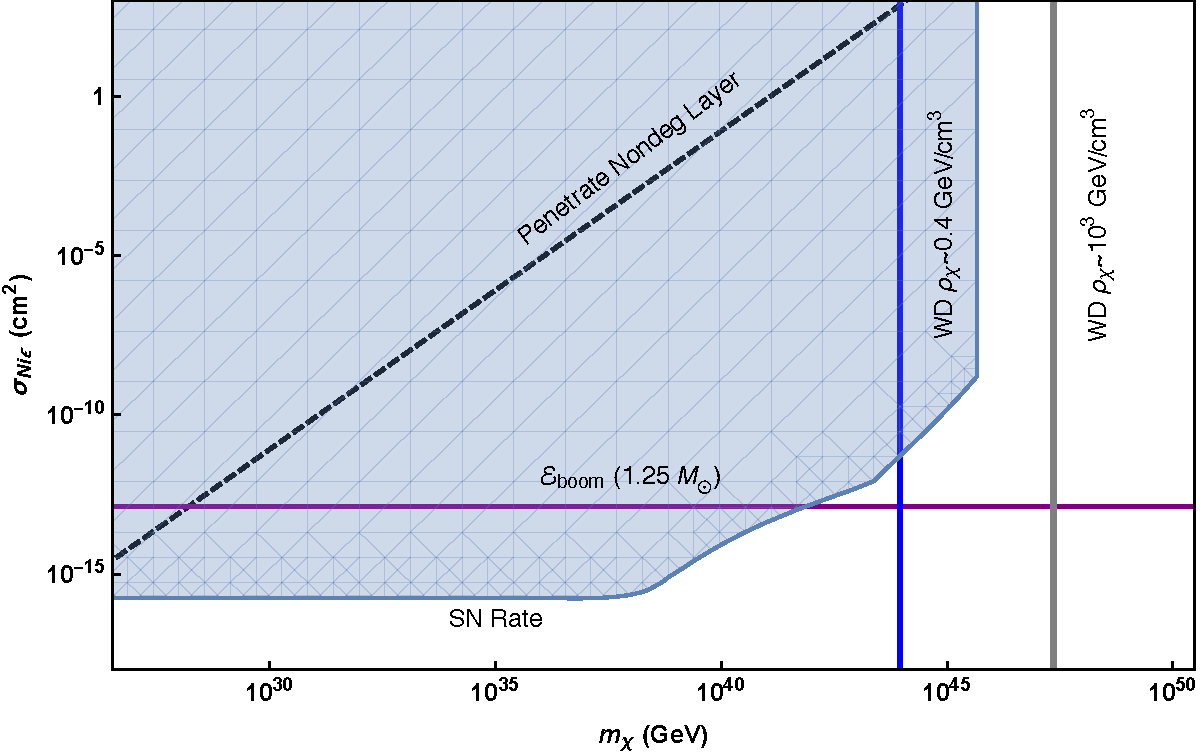
\includegraphics[scale=.35]{transitobservation.pdf}
\caption{Constraints on DM-nuclei inelastic scattering cross-section to produce a single SM product (e.g. photon) of energy $\epsilon = \text{TeV}$.
Bounds come from demanding that the DM transit triggers runaway fusion \eqref{eq:transitexplosion} (purple), occurs at a rate \eqref{eq:TransitRate} large enough to either ignite a single observed $1.25~M_{\astrosun}$ WD in its lifetime or exceed the measured SN rate in our galaxy (blue shaded). The dashed line is an example of the envelope-penetration constraint, assuming the energy deposit comes entirely from the DM's kinetic energy.
}
\label{fig:transit-inelastic}
\end{figure}

\subsection{Collision and Decay Constraints}
\label{sec:CollisionConstraints}

In order to constrain a DM model through its annihilations or decays within a WD, we require that it satisfy the ignition condition \eqref{eq:coldecay}.
Consider a simplified interaction wherein a single annihilation or decay releases $N$ particles of SM species $i$ and energy $\epsilon$.
Assuming a fractional parameter $f_\text{SM} = 1$, this corresponds to SM products with individual energy $\epsilon \sim m_\chi/N$.
Again, as long as $\epsilon \gg \MeV$ there is minimal dependence of the constraints on number of particles $N$ or species $i$ (with the exception of neutrinos).

With this schematic for the DM interaction, we can constrain the cross section for collision $\sigma_{\chi \chi}$ and lifetime $\tau_\chi$.
This is done in Figures~\ref{fig:transit-collision} and~\ref{fig:transit-decay} in the case of transiting DM using the different classes of observables for DM-DM collisions and DM decays, respectively.
In the case of captured DM, we also specify a benchmark value for the elastic scattering cross section $\sigma_{\chi A}$ and, with regards to DM-DM collisions, a stabilizing radius for the collapsing DM sphere.
This is done in Figures~\ref{fig:capture-collision} and~\ref{fig:capture-decay}---for simplicity, here we only show the constraints from the existence of nearby, heavy WDs.

\begin{figure}
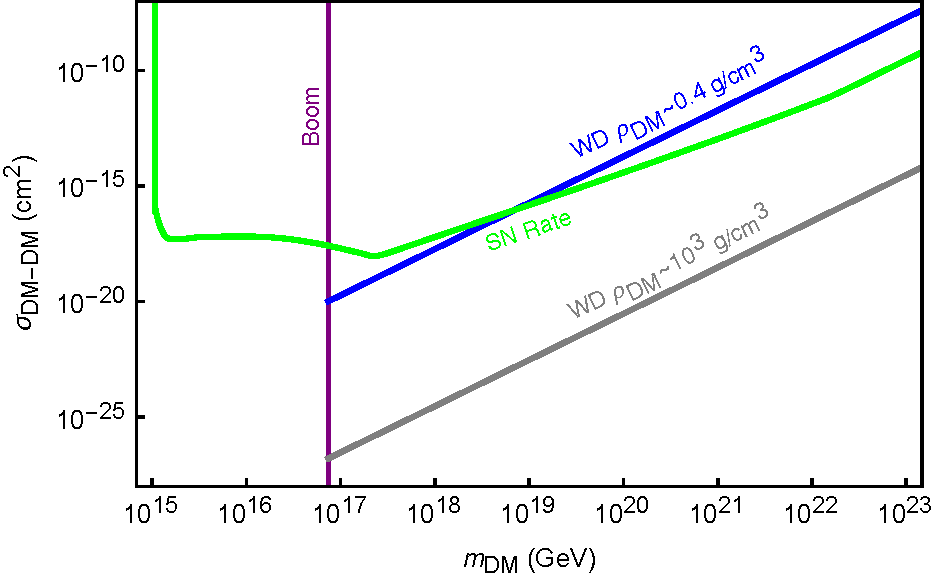
\includegraphics[scale=.35]{collisionobservation.pdf}
\caption{Constraints on DM-DM collision cross-section to SM products of energy $\epsilon \gg \MeV$.
Bounds come from demanding that the DM transit interaction triggers runaway fusion \eqref{eq:coldecay} (purple) and occurs at a rate \eqref{eq:collisionDM} large enough to either ignite a single observed $1.25~M_{\astrosun}$ WD in its lifetime or exceed the measured SN rate in our galaxy (blue shaded).
Also shown is the cosmological bound on DM self-interaction (red).}
\label{fig:transit-collision}
\end{figure}

\begin{figure}
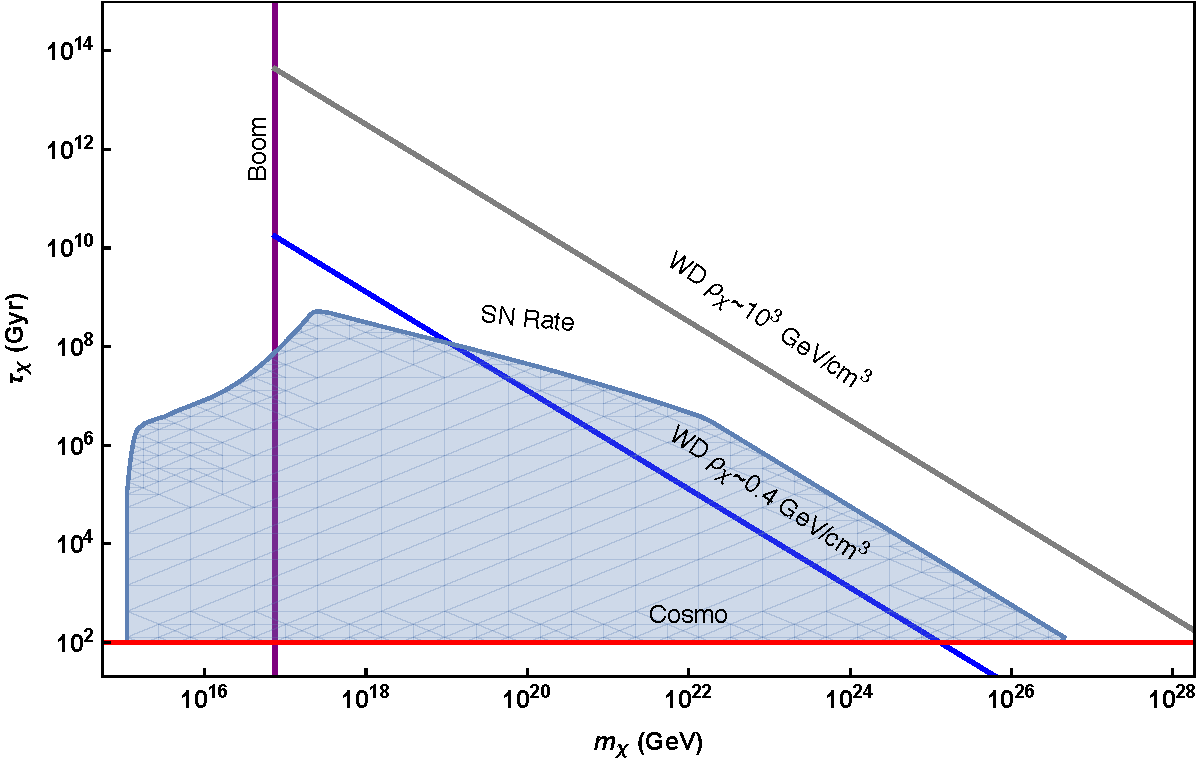
\includegraphics[scale=.35]{decayobservation.pdf}
\caption{Constraints on DM decay to SM products of energy $\epsilon \gg \MeV$.
Bounds come from demanding that the DM transit interaction triggers runaway fusion \eqref{eq:coldecay} (purple) and occurs at a rate \eqref{eq:decayDM} large enough to either ignite a single observed $1.25~M_{\astrosun}$ WD in its lifetime or exceed the measured SN rate in our galaxy (blue shaded).
Also shown is the cosmological bound on DM lifetime (red).}
\label{fig:transit-decay}
\end{figure}

\begin{figure}
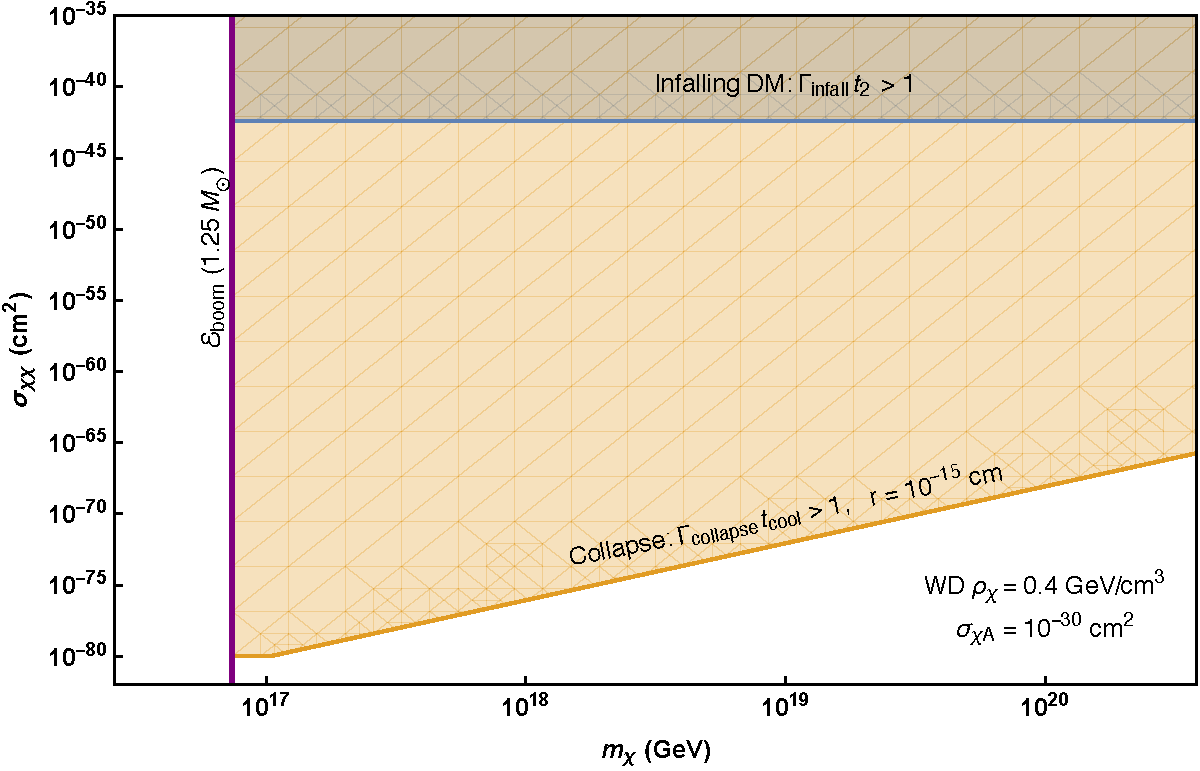
\includegraphics[scale=.35]{capturecollision.pdf}
\caption{Constraints on DM-DM collision cross-section to SM products of energy $\epsilon \gg \MeV$, assuming DM is captured with an elastic scattering $\sigma_{\chi A} = 10^{-30} ~\cm^2$.
Bounds come from the observation of a single $1.25~M_{\astrosun}$ WD in local DM density.
We consider the annihilation rate during the in-falling thermalization stage \eqref{eq:infall} (blue shaded) and during self-gravitational collapse \eqref{eq:collapse} to a stable radius $r = 10^{-15} ~\cm$ (orange shaded). See text for details.
}
\label{fig:capture-collision}
\end{figure}

\begin{figure}
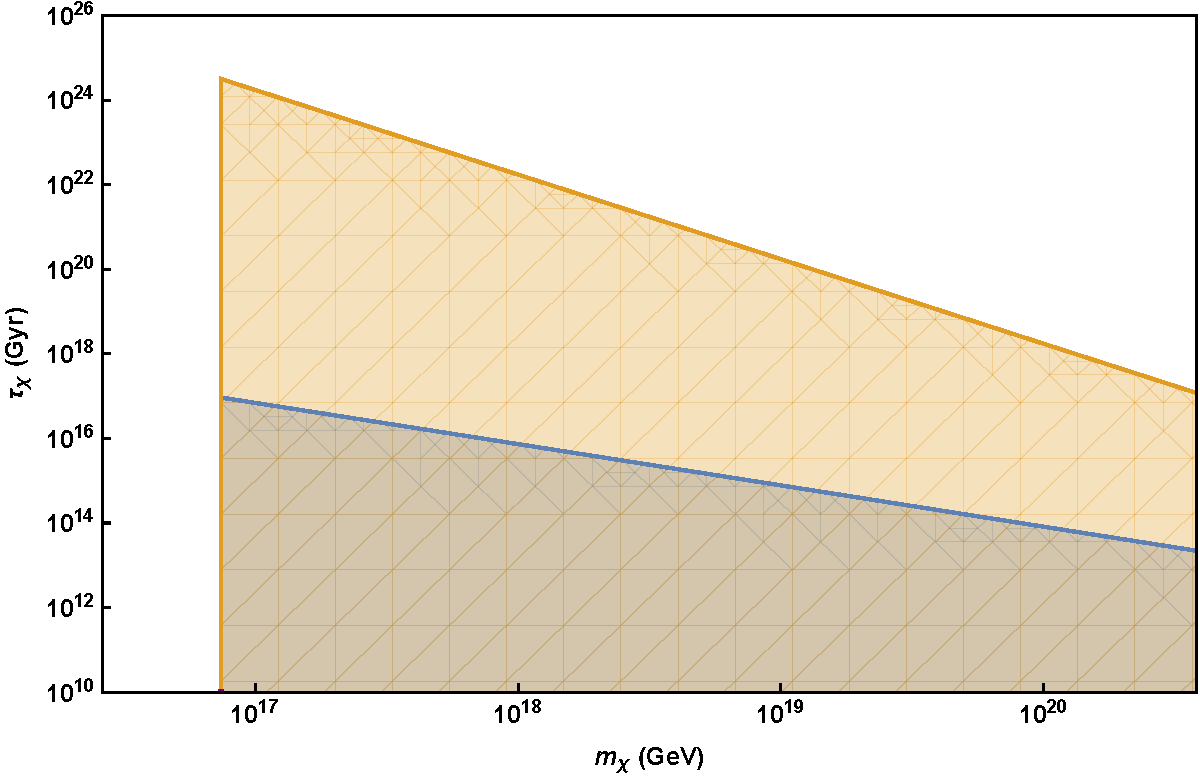
\includegraphics[scale=.35]{capturedecay.pdf}
\caption{Constraints on DM decay to SM products of energy $\epsilon \gg \MeV$, assuming DM is captured with an elastic scattering $\sigma_{\chi A} = 10^{-30} ~\cm^2$.
Bounds come from the observation of a single $1.25~M_{\astrosun}$ WD in local DM density.
We consider the decay rate during the in-falling thermalization stage \eqref{eq:decayDMcap} for gravitational collapse to a non-decaying DM core (blue shaded) or decaying DM core (orange shaded). See text for details.
}
\label{fig:capture-decay}
\end{figure}


Of course, there are additional limits on DM interactions of this kind complementary to the limits placed from WDs.
For one, demanding that the galactic halo has not substantially depleted during its lifetime yields a cosmological bound on DM self-interactions $\frac{\sigma_{\chi \chi}}{m_\chi} < \frac{\text{b}}{\GeV}$.
This is similar in magnitude to the bounds from colliding galaxy clusters \cite{Randall:2007ph}.
There is also a cosmological bound on DM lifetime $\tau_\chi > 100 ~\text{Gyr}$, independent of the nature of the decay products \cite{Poulin:2016nat}.
In addition, DM annihilations/decays in the galactic halo would contribute to the cosmic ray (CR) flux seen in terrestrial detectors.
As CRs of energy greater than $10^{12} ~\GeV$ have not yet been observed \cite{ThePierreAuger:2015rha, AbuZayyad:2012ru}, this places a bound on DM interaction parameters $\sigma_{\chi \chi}$ and $\tau_\chi$ which involve the release of such ultra-high energy particles.
The CR constraint on DM can be estimated by requiring that the expected time for an event to strike earth is less than the typical lifetime of a terrestrial detector $\sim 10 ~\text{yr}$.
For a detector of area $\sim (50~\text{km})^2$ \cite{ThePierreAuger:2015rha}, we find that the CR bounds are generally weaker than but within a few orders of magnitude of the WD bounds in the transit scenario.
This is actually due to a coincidence in the effective ``space-time volumes" of the two systems.
A CR detector sees events within a space-time volume $(R_\text{det}^2 R_\text{halo} \times 10 ~\text{yr})$ which is comparable to the WD space-time volume $(R_\text{WD}^3 \times 10^9 ~\text{yr})$, including the additional gravitational enhancement factors.
Note that a constraint can also be placed on lower-energy SM products from DM annihilations or decays which would provide an additional source for the measured CR flux, although such an analysis is beyond the scope of this work.
